\ifx\wholebook\relax \else
% ------------------------

\documentclass{article}
\usepackage[en]{../../../prelude}

\setcounter{page}{1}

\begin{document}

%--------------------------

% ================================================================
%                 COVER PAGE
% ================================================================

\title{Binary Heaps}

\author{Larry~LIU~Xinyu
\thanks{{\bfseries Larry LIU Xinyu } \newline
  Email: liuxinyu95@gmail.com \newline}
  }

\maketitle
\fi

\markboth{Binary Heaps}{Elementary Algorithms}

\ifx\wholebook\relax
\chapter{Binary Heaps}
\numberwithin{Exercise}{chapter}
\fi

% ================================================================
%                 Introduction
% ================================================================
\section{Introduction}
\label{introduction}
\index{Binary heap}

Heaps are one of the most widely used data structures--used
to solve practical problems such as sorting, prioritized
scheduling and in implementing graph algorithms, to name a few\cite{wiki-heap}.

Most popular implementations of heaps use a kind of implicit
binary heap using arrays, which is described in \cite{CLRS}.
Examples include C++/STL heap and Python heapq. The most efficient
heap sort algorithm is also
realized with binary heap as proposed by R. W. Floyd
\cite{wiki-heapsort} \cite{rosetta-heapsort}.

However, heaps can be general and realized with varies
of other data structures besides array.
In this chapter, explicit
binary tree is used. It leads to Leftist heaps, Skew heaps,
and Splay heaps, which are suitable for purely functional
implementation as shown
by Okasaki\cite{okasaki-book}.

A heap is a data structure that satisfies the following {\em heap property}.
\begin{itemize}
\item Top operation always returns the minimum (maximum) element;
\item Pop operation removes the top element from the heap while the heap
property should be kept, so that the new top element is still the
minimum (maximum) one;
\item Insert a new element to heap should keep the heap property. That
the new top is still the minimum (maximum) element;
\item Other operations including merge etc should all keep the heap property.
\end{itemize}

This is a kind of recursive definition, while it doesn't limit the under
ground data structure.

We call the heap with the minimum element on top as {\em min-heap},
while if the top keeps the maximum element, we call it {\em max-heap}.

% ================================================================
%                 Implicit binary heap by array
% ================================================================
\section{Implicit binary heap by array}
\label{ibheap}
\index{Implicit binary heap}

Considering the heap definition in previous section, one option to
implement heap is by using trees. A straightforward solution is
to store the minimum (maximum) element in the root of the
tree, so for `top' operation, we simply return the root as the
result. And for `pop' operation, we can remove the root and
rebuild the tree from the children.

If binary tree is used to implement the heap, we
can call it {\em binary heap}. This chapter explains three different
realizations for binary heap.

% ================================================================
%                 Definition
% ================================================================
\subsection{Definition}

The first one is implicit binary tree. Consider the problem
how to represent a complete binary tree with array. (For example, try to
represent a complete binary tree in the programming language doesn't support structure
or record data type. Only array can be used). One solution
is to pack all elements from top level (root) down to bottom level (leaves).

Figure \ref{fig:tree-array-map} shows a complete binary tree and
its corresponding array representation.

\begin{figure}[htbp]
       \begin{center}
       	  \includegraphics[scale=0.5]{img/tree-array-map-tree.ps}
          \includegraphics[scale=0.5]{img/tree-array-map-array.ps}
        \caption{Mapping between a complete binary tree and array} \label{fig:tree-array-map}
       \end{center}
\end{figure}

This mapping between tree and array can be defined as
the following equations (The array index starts from 1).

\begin{algorithmic}[1]
\Function{Parent}{$i$}
  \State \Return $\lfloor \frac{i}{2} \rfloor$
\EndFunction
\Statex
\Function{Left}{$i$}
  \State \Return $2i$
\EndFunction
\Statex
\Function{Right}{$i$}
  \State \Return $2i+1$
\EndFunction
\end{algorithmic}

For a given tree node which is represented as the $i$-th element of the
array, since the tree is complete, we can easily find its parent node
as the $\lfloor i/2 \rfloor$-th element; Its left child
with index of $2i$ and right child of $2i+1$. If the index
of the child exceeds the length of the array, it means this
node does not have such a child (leaf for example).

In real implementation, this mapping can be calculated fast
with bit-wise operation like the following example ANSI C code.
Note that, the array index starts from zero in C like
languages.

\lstset{language=C}
\begin{lstlisting}
#define PARENT(i) ((((i) + 1) >> 1) - 1)

#define LEFT(i) (((i) << 1) + 1)

#define RIGHT(i) (((i) + 1) << 1)
\end{lstlisting}

% ================================================================
%                 Heapify
% ================================================================
\subsection{Heapify}
\index{Binary heap!Heapify}

The most important thing for heap algorithm is to maintain the heap
property, that the top element should be the minimum (maximum) one.

For the implicit binary heap by array, it means for a given node,
which is represented as the $i$-th index, we can develop a method
to check if both its two children are not less than the parent. In case
there is violation, we need swap the parent and child recursively \cite{CLRS}.
Note that here we assume both the two sub-trees are the valid heaps.

Below algorithm shows the iterative solution to enforce the min-heap
property from a given index of the array.

\begin{algorithmic}[1]
\Function{Heapify}{$A, i$}
  \State $n \gets |A|$
  \Loop
    \State $l \gets$ \Call{Left}{$i$}
    \State $r \gets$ \Call{Right}{$i$}
    \State $smallest \gets i$
    \If{$l < n \land A[l] < A[i]$}
      \State $smallest \gets l$
    \EndIf
    \If{$r < n \land A[r] < A[smallest]$}
      \State $smallest \gets r$
    \EndIf
    \If{$smallest \neq i$}
      \State \textproc{Exchange} $A[i] \leftrightarrow A[smallest]$
      \State $i \gets smallest$
    \Else
      \State \Return
    \EndIf
  \EndLoop
\EndFunction
\end{algorithmic}

For array $A$ and the given index $i$, None its children
should be less than $A[i]$, in case there is violation, we pick the smallest
element as $A[i]$, and swap the previous $A[i]$ to child.
The algorithm traverses the tree top-down to fix the heap property
until either reach a leaf or there is no heap property violation.

The \textproc{Heapify} algorithm takes $O(\lg n)$ time, where
$n$ is the number of elements. This
is because the loop time is proportion to the height of the complete binary tree.

When implement this algorithm, the comparison method can be passed as
a parameter, so that both min-heap and max-heap can be supported.
The following ANSI C example code uses this approach.

\begin{lstlisting}
typedef int (*Less)(Key, Key);
int less(Key x, Key y) { return x < y; }
int notless(Key x, Key y) { return !less(x, y); }

void heapify(Key* a, int i, int n, Less lt) {
    int l, r, m;
    while (1) {
        l = LEFT(i);
        r = RIGHT(i);
        m = i;
        if (l < n && lt(a[l], a[i]))
            m = l;
        if (r < n && lt(a[r], a[m]))
            m = r;
        if (m != i) {
            swap(a, i, m);
            i = m;
        } else
            break;
    }
}
\end{lstlisting}

Figure \ref{fig:heapify} illustrates the steps when \textproc{Heapify} processing the
array $\{16, 4, 10, 14, 7, 9, 3, 2, 8, 1\}$ from the second index. The array changes to
$\{16, 14, 10, 8, 7, 9, 3, 2, 4, 1\}$ as a max-heap.

\begin{figure}[htbp]
    \centering
    \subfloat[Step 1, 14 is the biggest element among 4, 14, and 7. Swap 4 with the left child;]{\includegraphics[scale=0.5]{img/heapify-1.ps}} \\
    \subfloat[Step 2, 8 is the biggest element among 2, 4, and 8. Swap 4 with the right child;]{\includegraphics[scale=0.5]{img/heapify-2.ps}} \\
    \subfloat[4 is the leaf node. It hasn't any children. Process terminates.]{\includegraphics[scale=0.5]{img/heapify-3.ps}}
    \caption{Heapify example, a max-heap case.} \label{fig:heapify}
\end{figure}


% ================================================================
%                 Build a heap
% ================================================================
\subsection{Build a heap}
\index{Binary heap!build heap}

With \textproc{Heapify} algorithm defined, it is easy to build a heap from an arbitrary
array. Observe that the numbers of nodes in a complete binary tree
for each level is a list like below:

$1, 2, 4, 8, ..., 2^i, ...$.

The only exception is the last level. Since the tree may not full
(note that complete binary tree doesn't mean full binary tree), the
last level contains at most $2^{p-1}$ nodes, where $2^p + 1 \leq n$ and $n$
is the length of the array.

The \textproc{Heapify} algorithm doesn't have any effect on leave node.
We can skip applying \textproc{Heapify} for all leaves. In other words,
all leaf nodes have already satisfied the heap property. We only need
start checking and maintain the heap property from the last branch node.
the index of the last branch node is no greater than $\lfloor n/2 \rfloor$.

Based on this fact, we can build a heap with the following algorithm.
(Assume the heap is min-heap).

\begin{algorithmic}[1]
\Function{Build-Heap}{$A$}
  \State $n \gets |A|$
  \For{$i \gets \lfloor n/2 \rfloor$ down to $1$}
    \State \Call{Heapify}{$A, i$}
  \EndFor
\EndFunction
\end{algorithmic}

Although the complexity of \textproc{Heapify} is $O(\lg n)$, the running time
of \textproc{Build-Heap} is not bound to $O(n \lg n)$ but $O(n)$. It
is a linear time algorithm. This can be deduced as the following:

The heap is built by skipping all leaves.
Given $n$ nodes, there are at most $n/4$ nodes being compared and moved down 1 time;
at most $n/8$ nodes being compared and moved down 2 times; at most $n/16$ nodes being
compared and moved down 3 times,... Thus the upper bound of total comparison and
moving time is:

\be
S = n (\frac{1}{4} + 2 \frac{1}{8} + 3 \frac{1}{16} + ...)
\label{eq:build-heap-1}
\ee

Times by 2 for both sides, we have:

\be
2S = n (\frac{1}{2} + 2 \frac{1}{4} + 3 \frac{1}{8} + ...)
\label{eq:build-heap-2}
\ee

Substract equation (\ref{eq:build-heap-1}) from (\ref{eq:build-heap-2}):

\[
S = n (\frac{1}{2} + \frac{1}{4} + \frac{1}{8} + ...) = n
\]

Below ANSI C example program implements this heap building function.

\lstset{language=C}
\begin{lstlisting}
void build_heap(Key* a, int n, Less lt) {
    int i;
    for (i = (n-1) >> 1; i >= 0; --i)
        heapify(a, i, n, lt);
}
\end{lstlisting}

Figure \ref{fig:build-heap-1}, \ref{fig:build-heap-2} and \ref{fig:build-heap-3}
show the steps when building a max-heap from
array $\{4, 1, 3, 2, 16, 9, 10, 14, 8, 7\}$.
The node in black color is the one where \textproc{Heapify} being
applied, the nodes in gray color are swapped in order to keep the heap property.

\begin{figure}[htbp]
    \centering
    \subfloat[An array in arbitrary order before heap building process;]{\includegraphics[scale=0.5]{img/build-heap-array.ps}} \\
    \subfloat[Step 1, The array is mapped to binary tree. The first branch node, which is
16 is examined;]{\includegraphics[scale=0.5]{img/build-heap-1.ps}} \\
    \subfloat[Step 2, 16 is the largest element in current sub tree, next is to check node
with value 2;]{\includegraphics[scale=0.5]{img/build-heap-2.ps}}
    \caption{Build a heap from the arbitrary array. Gray nodes are changed in each step,
black node will be processed next step.} \label{fig:build-heap-1}
\end{figure}

\begin{figure}[htbp]
    \centering
    \subfloat[Step 3, 14 is the largest value in the sub-tree, swap 14 and 2; next is to check
node with value 3;]{\includegraphics[scale=0.5]{img/build-heap-3.ps}} \\
    \subfloat[Step 4, 10 is the largest value in the sub-tree, swap 10 and 3; next is to check
node with value 1;]{\includegraphics[scale=0.5]{img/build-heap-4.ps}}
    \caption{Build a heap from the arbitrary array. Gray nodes are changed in each step,
black node will be processed next step.} \label{fig:build-heap-2}
\end{figure}

\begin{figure}[htbp]
    \centering
    \subfloat[Step 5, 16 is the largest value in current sub-tree, swap 16 and 1 first; then
similarly, swap 1 and 7; next is to check the root node with value 4;]{\includegraphics[scale=0.5]{img/build-heap-5.ps}} \\
    \subfloat[Step 6, Swap 4 and 16, then swap 4 and 14, and then swap 4 and 8;
And the whole build process finish.]{\includegraphics[scale=0.5]{img/build-heap-6.ps}}
    \caption{Build a heap from the arbitrary array. Gray nodes are changed in each step,
black node will be processed next step.} \label{fig:build-heap-3}
\end{figure}

% ================================================================
%                 Basic heap operations
% ================================================================
\subsection{Basic heap operations}

The generic definition of heap (not necessarily the binary heap)
demands us to to provide basic operations for accessing and modifying data.

The most important operations include accessing the top element
(find the minimum or maximum one), popping the top element
from the heap, finding the top $k$ elements, decreasing a key (
for min-heap. It is increasing a key for max-heap), and
insertion.

For the binary tree, most of operations are bound to $O(\lg n)$ in
worst-case, some of them, such as top is $O(1)$ constant time.

\subsubsection{Access the top element}
\index{Binary heap!top}
For the binary tree realization, it is the
root stores the minimum (maximum) value. This is the first
element in the array.

\begin{algorithmic}[1]
\Function{Top}{$A$}
  \State \Return $A[1]$
\EndFunction
\end{algorithmic}

This operation is trivial. It takes $O(1)$ time.
Here we skip the error handling for empty case. If the
heap is empty, one option is to raise an error.

\subsubsection{Heap Pop}
\index{Binary heap!pop}

Pop operation is more
complex than accessing the top, because the heap property has to be maintained
after the top element is removed.

The solution is to apply \textproc{Heapify} algorithm to the
next element after the root is removed.

One simple but slow method based on this idea looks like
the following.

\begin{algorithmic}[1]
\Function{Pop-Slow}{$A$}
  \State $x \gets$ \Call{Top}{$A$}
  \State \Call{Remove}{$A$, 1}
  \If{$A$ is not empty}
    \State \Call{Heapify}{$A$, 1}
  \EndIf
  \State \Return $x$
\EndFunction
\end{algorithmic}

This algorithm firstly records the top element in $x$, then
it removes the first element from the array, the size of
this array is reduced by one. After that if the array isn't
empty, \textproc{Heapify} will applied to the new array from
the first element (It was previously the second one).

Removing the first element from array takes $O(n)$ time,
where $n$ is the length of the array. This is because
we need shift all the rest elements one by one.
This bottle neck slows the whole algorithm
to linear time.

In order to solve this problem, one alternative is
to swap the first element with the last one in the
array, then shrink the array size by one.

\begin{algorithmic}[1]
\Function{Pop}{$A$}
  \State $x \gets$ \Call{Top}{$A$}
  \State $n \gets$ \Call{Heap-Size}{$A$}
  \State \textproc{Exchange} $A[1] \leftrightarrow A[n]$
  \State \Call{Remove}{$A, n$}
  \If{$A$ is not empty}
    \State \Call{Heapify}{$A$, 1}
  \EndIf
  \State \Return $x$
\EndFunction
\end{algorithmic}

Removing the last element from the array takes
only constant $O(1)$ time, and \textproc{Heapify} is bound to $O(\lg n)$.
Thus the whole algorithm performs in $O(\lg n)$ time. The following
example ANSI C program implements this algorithm\footnote{This program does not
actually remove the last element, it reuse the last cell to store the popped
result}.

\lstset{language=C}
\begin{lstlisting}
Key pop(Key* a, int n, Less lt) {
    swap(a, 0, --n);
    heapify(a, 0, n, lt);
    return a[n];
}
\end{lstlisting}

\subsubsection{Find the top $k$ elements}
\index{Binary heap!top-k}

With pop defined, it is easy to
find the top $k$ elements from array.
we can build a max-heap from the array, then perform
pop operation $k$ times.

\begin{algorithmic}[1]
\Function{Top-k}{$A, k$}
  \State $R \gets \phi$
  \State \Call{Build-Heap}{$A$}
  \For{$i \gets 1$ to \textproc{Min}(k, |$A$|)}
    \State \textproc{Append}($R$, \Call{Pop}{$A$})
  \EndFor
  \State \Return $R$
\EndFunction
\end{algorithmic}

If $k$ is greater than the length of the array,
we need return the whole array as the result. That's why it calls
the \textproc{Min} function to determine the number of loops.

Below example Python program implements the top-$k$ algorithm.

\lstset{language=Python}
\begin{lstlisting}
def top_k(x, k, less_p = MIN_HEAP):
    build_heap(x, less_p)
    return [heap_pop(x, less_p) for _ in range(min(k, len(x)))]
\end{lstlisting}

\subsubsection{Decrease key}
\index{Binary heap!decrease key}

Heap can be used to implement priority queue. It
is important to support key modification in heap. One typical operation
is to increase the priority of a tasks so that it can be performed
earlier.

Here we present the decrease key operation for a min-heap. The
corresponding operation is increase key for max-heap.
Figure \ref{fig:decrease-key-1} and \ref{fig:decrease-key-2} illustrate such a case for a max-heap.
The key of the 9-th node is increased from 4 to 15.

\begin{figure}[htbp]
    \centering
    \subfloat[The 9-th node with key 4 will be modified;]{\includegraphics[scale=0.5]{img/decrease-key-a.ps}} \\
    \subfloat[The key is modified to 15, which is greater than its parent;]{\includegraphics[scale=0.5]{img/decrease-key-b.ps}} \\
    \subfloat[According the max-heap property, 8 and 15 are swapped.]{\includegraphics[scale=0.5]{img/decrease-key-c.ps}}
    \caption{Example process when increase a key in a max-heap.} \label{fig:decrease-key-1}
\end{figure}

\begin{figure}[htbp]
    \centering
    \subfloat[Since 15 is greater than its parent 14, they are swapped. After that, because 15 is less than 16, the process terminates.]{\includegraphics[scale=0.5]{img/decrease-key-d.ps}}
    \caption{Example process when increase a key in a max-heap.} \label{fig:decrease-key-2}
\end{figure}

Once a key is decreased in a min-heap, it may make
the node conflict with the heap property, that the key may be less
than some ancestor. In order to maintain the
invariant, the following auxiliary algorithm is defined to resume the heap
property.

\begin{algorithmic}[1]
\Function{Heap-Fix}{$A, i$}
  \While{$i>1 \land A[i] < A[$ \Call{Parent}{$i$} $]$}
    \State \textproc{Exchange} $A[i] \leftrightarrow A[$ \Call{Parent}{$i$} $]$
    \State $i \gets$  \Call{Parent}{$i$}
  \EndWhile
\EndFunction
\end{algorithmic}

This algorithm repeatedly compares the keys of parent node and
current node. It swap the nodes if
the parent contains the smaller key. This process is performed
from the current node towards the root node till it finds that
the parent node holds the smaller key.

With this auxiliary algorithm, decrease key can be realized
as below.

\begin{algorithmic}[1]
\Function{Decrease-Key}{$A, i, k$}
  \If{$k < A[i]$}
    \State $A[i] \gets k$
    \State \Call{Heap-Fix}{$A, i$}
  \EndIf
\EndFunction
\end{algorithmic}

This algorithm is only triggered when the new key
is less than the original key. The performance is bound to $O(\lg n)$.
Below example ANSI C program implements the algorithm.

\lstset{language=C}
\begin{lstlisting}
void heap_fix(Key* a, int i, Less lt) {
    while (i > 0 && lt(a[i], a[PARENT(i)])) {
        swap(a, i, PARENT(i));
        i = PARENT(i);
    }
}

void decrease_key(Key* a, int i, Key k, Less lt) {
    if (lt(k, a[i])) {
        a[i] = k;
        heap_fix(a, i, lt);
    }
}
\end{lstlisting}

\subsubsection{Insertion}
\index{Binary heap!insertion}
\index{Binary heap!heap push}

Insertion can be implemented by using \textproc{Decrease-Key} \cite{CLRS}.
A new node with $\infty$ as key is created. According
to the min-heap property, it should be the last element
in the under ground array. After that, the key is decreased to
the value to be inserted, and \textproc{Decrease-Key} is called
to fix any violation to the heap property.

Alternatively, we can reuse \textproc{Heap-Fix} to implement
insertion. The new key is directly appended at the end of the array,
and the \textproc{Heap-Fix} is applied to this new node.

\begin{algorithmic}[1]
\Function{Heap-Push}{$A, k$}
  \State \Call{Append}{$A, k$}
  \State \Call{Heap-Fix}{$A, |A|$}
\EndFunction
\end{algorithmic}

The following example Python program implements the heap insertion
algorithm.

\lstset{language=Python}
\begin{lstlisting}
def heap_insert(x, key, less_p = MIN_HEAP):
    i = len(x)
    x.append(key)
    heap_fix(x, i, less_p)
\end{lstlisting}

% ================================================================
%                 Heap sort
% ================================================================
\subsection{Heap sort}
\label{heap-sort}
\index{Heap sort}

Heap sort is interesting application of heap. According
to the heap property, the min(max) element can be easily accessed
by from the top of the heap. A straightforward way to sort a list
of values is to build a heap from them, then continuously
pop the smallest element till the heap is empty.

The algorithm based on this idea can be defined like below.

\begin{algorithmic}[1]
\Function{Heap-Sort}{$A$}
  \State $R \gets \phi$
  \State \Call{Build-Heap}{$A$}
  \While{$A \neq \phi$}
    \State \textproc{Append}($R$, \Call{Heap-Pop}{$A$})
  \EndWhile
  \State \Return $R$
\EndFunction
\end{algorithmic}

The following Python example program implements this definition.

\lstset{language=Python}
\begin{lstlisting}
def heap_sort(x, less_p = MIN_HEAP):
    res = []
    build_heap(x, less_p)
    while x!=[]:
        res.append(heap_pop(x, less_p))
    return res
\end{lstlisting}

When sort $n$ elements, the \textproc{Build-Heap} is bound to $O(n)$.
Since pop is $O(\lg n)$, and it
is called $n$ times, so the overall sorting takes $O(n \lg n)$
time to run. Because we use another list to hold the result,
the space requirement is $O(n)$.

Robert. W. Floyd found a fast implementation of heap sort.
The idea is to build a max-heap instead of min-heap, so the first
element is the biggest one. Then the biggest element is swapped
with the last element in the array, so that it is in the right
position after sorting. As the last element becomes the new top,
it may violate the heap property. We can shrink the heap size
by one and perform
\textproc{Heapify} to resume the heap property.
This process
is repeated till there is only one element left in the heap.

\begin{algorithmic}[1]
\Function{Heap-Sort}{$A$}
  \State \Call{Build-Max-Heap}{$A$}
  \While{$|A| > 1$}
    \State \textproc{Exchange} $A[1] \leftrightarrow A[n]$
    \State $|A| \gets |A| - 1$
    \State \Call{Heapify}{$A, 1$}
  \EndWhile
\EndFunction
\end{algorithmic}

This is in-place algorithm, it needn't any extra spaces to hold
the result. The following ANSI C example code
implements this algorithm.

\lstset{language=C}
\begin{lstlisting}
void heap_sort(Key* a, int n) {
    build_heap(a, n, notless);
    while(n > 1) {
        swap(a, 0, --n);
        heapify(a, 0, n, notless);
    }
}
\end{lstlisting}

\begin{Exercise}
\begin{itemize}
\item Somebody considers one alternative to realize in-place heap sort. Take
sorting the array in ascending order as example, the first step is to build
the array as a minimum heap $A$, but not the maximum heap like the Floyd's method.
After that the first element $a_1$ is in the correct place. Next, treat
the rest $\{a_2, a_3, ..., a_n\}$ as a new heap, and perform
\textproc{Heapify} to them from $a_2$ for these $n-1$ elements. Repeating this
advance and \textproc{Heapify} step from left to right would sort the array.
The following example ANSI C code illustrates this idea.
Is this solution correct? If yes, prove it; if not, why?
\lstset{language=C}
\begin{lstlisting}
void heap_sort(Key* a, int n) {
    build_heap(a, n, less);
    while(--n)
        heapify(++a, 0, n, less);
}
\end{lstlisting}

\item Because of the same reason, can we perform \textproc{Heapify} from
left to right $k$ times to realize in-place top-$k$ algorithm like below
ANSI C code?
\lstset{language=C}
\begin{lstlisting}
int tops(int k, Key* a, int n, Less lt) {
    build_heap(a, n, lt);
    for (k = MIN(k, n) - 1; k; --k)
        heapify(++a, 0, --n, lt);
    return k;
}
\end{lstlisting}
\end{itemize}
\end{Exercise}

% ================================================================
%                 Explicit binary heap
% ================================================================
\section{Leftist heap and Skew heap, the explicit binary heaps}
\label{ebheap}

Instead of using implicit binary tree by array, it is natural to
consider why we can't use explicit binary tree to realize heap?

There are some problems must be solved if we turn into explicit
binary tree as the under ground data structure.

The first problem is about the \textproc{Heap-Pop} or \textproc{Delete-Min} operation.
Consider the binary tree is represented in form of left, key, and right as
$(L, k, R)$, which is shown in figure \ref{fig:lvr}

\begin{figure}[htbp]
    \centering
    \includegraphics[scale=0.8]{img/lvr.ps}
    \caption{A binary tree, all elements in children are not less than $k$.} \label{fig:lvr}
\end{figure}

If $k$ is the top element, all elements in left and right children are not less
than $k$ in a min-heap. After $k$ is popped, only left and right children are left.
They have to be merged to a new tree. Since heap property should be maintained
after merge, the new root is still the smallest element.

Because both left and right children are binary trees conforming heap property,
the two trivial cases can be defined immediately.

\[
merge(H_1, H_2) = \left \{
  \begin{array}
  {r@{\quad:\quad}l}
  H_2 & H_1 = \phi \\
  H_1 & H_2 = \phi \\
  ? & otherwise
  \end{array}
\right.
\]

Where $\phi$ means empty heap.

If neither left nor right child is empty, because they all fit
heap property, the top elements of them are all the minimum respectively.
We can compare these two roots,
and select the smaller as the new root of the merged heap.

For instance, let $L = (A, x, B)$ and $R = (A', y, B')$, where $A$, $A'$, $B$,
and $B'$ are all sub trees. If $x < y$, $x$ will be the new root.
We can either keep $A$, and recursively merge $B$ and $R$; or
keep $B$, and merge $A$ and $R$, so the new heap can be one
of the following.

\begin{itemize}
\item $(merge(A, R), x, B)$
\item $(A, x, merge(B, R))$
\end{itemize}

Both are correct. One simplified solution is to only merge the right
sub tree. {\em Leftist} tree provides a systematically approach based on this
idea.

% ================================================================
%                 Definition
% ================================================================
\subsection{Definition}
\index{Leftist heap}

The heap implemented by Leftist tree is called Leftist heap. Leftist
tree is first introduced by C. A. Crane in 1972\cite{wiki-leftist-tree}.

\subsubsection{Rank (S-value)}
\index{Leftist heap!rank}
\index{Leftist heap!S-value}

In Leftist tree, a rank value (or $S$ value) is defined for each node.
Rank is the distance to the nearest external node. Where external node
is the NIL concept extended from the leaf node.

For example, in figure \ref{fig:rank}, the rank of NIL
is defined 0, consider the root node 4, The nearest external node is
the child of node 8. So the rank of root node 4 is 2. Because node
6 and node 8 both only contain NIL, so their rank values are 1.
Although node 5 has non-NIL left child, However, since the right
child is NIL, so the rank value, which is the minimum distance
to NIL is still 1.

\begin{figure}[htbp]
   \begin{center}
     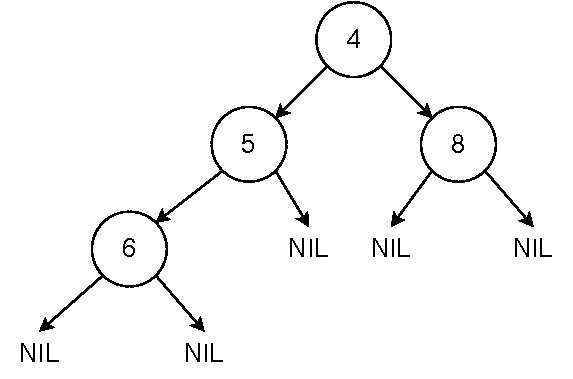
\includegraphics[scale=0.5]{img/rank.ps}
     \caption{$rank(4) = 2$, $rank(6) = rank(8) = rank(5) = 1$.} \label{fig:rank}
   \end{center}
\end{figure}

\subsubsection{Leftist property}

With rank defined, we can create a strategy when merging.

\begin{itemize}
\item Every time when merging, we always merge to right child; Denote the rank
of the new right sub tree as $r_r$;
\item Compare the ranks of the left and right children, if the rank of
left sub tree is $r_l$ and $r_l < r_r$, we swap the left and the right children.
\end{itemize}

We call this `Leftist property'. In general, a Leftist tree always
has the shortest path to some external node on the right.

Leftist tree tends to be very unbalanced, However, it ensures important
property as specified in the following theorem.

\begin{theorem}
If a Leftist tree $T$ contains $n$ internal nodes, the path from root to the
rightmost external node contains at most $\lfloor \log (n+1) \rfloor$ nodes.
\end{theorem}

We skip the proof here, readers can refer to \cite{brono-book} and \cite{TAOCP}
for more information. With this theorem, algorithms operate along this path are
all bound to $O(\lg n)$.

We can reuse the binary tree definition, and augment with a rank field to
define the Leftist tree, for example in form of $(r, k, L, R)$ for non-empty
case. Below Haskell code defines the Leftist tree.

\lstset{language=Haskell}
\begin{lstlisting}
data LHeap a = E -- Empty
             | Node Int a (LHeap a) (LHeap a) -- rank, element, left, right
\end{lstlisting}

For empty tree, the rank is defined as zero. Otherwise, it's the value
of the augmented field. A $rank(H)$ function can be
given to cover both cases.

\be
rank(H) = \left \{
  \begin{array}
  {r@{\quad:\quad}l}
  0 & H = \phi \\
  r & otherwise, H = (r, k, L, R)
  \end{array}
\right.
\ee

Here is the example Haskell rank function.

\lstset{language=Haskell}
\begin{lstlisting}
rank E = 0
rank (Node r _ _ _) = r
\end{lstlisting}

In the rest of this section, we denote $rank(H)$ as $r_H$

% ================================================================
%                 Merge
% ================================================================
\subsection{Merge}
\index{Leftist heap!merge}

In order to realize `merge', we need develop the auxiliary algorithm
to compare the ranks and swap the children if necessary.

\be
mk(k, A, B) = \left \{
  \begin{array}
  {r@{\quad:\quad}l}
  (r_A + 1, k, B, A) & r_A < r_B \\
  (r_B + 1, k, A, B) & otherwise
  \end{array}
\right.
\ee

This function takes three arguments, a key and two sub trees $A$, and $B$.
if the rank of $A$ is smaller, it builds a bigger tree with $B$ as the left child,
and $A$ as the right child. It increment the rank of $A$ by 1 as the
rank of the new tree; Otherwise if $B$ holds the smaller rank, then $A$ is
set as the left child, and $B$ becomes the right. The resulting rank
is $r_b + 1$.

The reason why rank need be increased by one is because there
is a new key added on top of the tree. It causes the rank
increasing.

Denote the key, the left and right children for $H_1$ and $H_2$ as
$k_1, L_1, R_1$, and $k_2, L_2, R_2$ respectively.
The $merge(H_1, H_2)$ function can be completed by using this auxiliary
tool as below

\be
merge(H_1, H_2) = \left \{
  \begin{array}
  {r@{\quad:\quad}l}
  H_2 & H_1 = \phi \\
  H_1 & H_2 = \phi \\
  mk(k_1, L_1, merge(R_1, H_2)) & k_1 < k_2 \\
  mk(k_2, L_2, merge(H_1, R_2)) & otherwise
  \end{array}
\right.
\ee

The $merge$ function is always recursively called on the right side,
and the Leftist property is maintained. These facts ensure the performance
being bound to $O(\lg n)$.

The following Haskell example code implements the merge program.

\lstset{language=Haskell}
\begin{lstlisting}
merge E h = h
merge h E = h
merge h1@(Node _ x l r) h2@(Node _ y l' r') =
    if x < y then makeNode x l (merge r h2)
    else makeNode y l' (merge h1 r')

makeNode x a b = if rank a < rank b then Node (rank a + 1) x b a
                 else Node (rank b + 1) x a b
\end{lstlisting}

\subsubsection{Merge operation in implicit binary heap by array}
\index{Binary heap!merge}

Implicit binary heap by array performs very fast in most cases, and
it fits modern computer with cache technology well. However, merge
is the algorithm bounds to $O(n)$ time. The typical realization is to
concatenate two arrays together and make a heap for this array \cite{NIST}.

\begin{algorithmic}[1]
\Function{Merge-Heap}{$A, B$}
  \State $C \gets$ \Call{Concat}{$A, B$}
  \State \Call{Build-Heap}{$C$}
\EndFunction
\end{algorithmic}

% ================================================================
%                 Basic heap operations
% ================================================================
\subsection{Basic heap operations}

Most of the basic heap operations can be implemented with $merge$
algorithm defined above.

\subsubsection{Top and pop}
\index{Leftist heap!top}
\index{Leftist heap!pop}
Because the smallest element is always held in root, it's trivial
to find the minimum value. It's constant $O(1)$ operation. Below
equation extracts the root from non-empty heap $H = (r, k, L, R)$.
The error handling for empty case is skipped here.

\be
top(H) = k
\ee

For pop operation, firstly, the top element is removed, then
left and right children are merged to a new heap.

\be
pop(H) = merge(L, R)
\ee

Because it calls $merge$ directly, the pop operation on Leftist heap is bound
to $O(\lg n)$.

\subsubsection{Insertion}
\index{Leftist heap!insertion}

To insert a new element, one solution is to create a single
leaf node with the element, and then merge this leaf node to
the existing Leftist tree.

\be
insert(H, k) = merge(H, (1, k, \phi, \phi))
\ee

It is $O(\lg n)$ algorithm since insertion also calls $merge$ directly.

There is a convenient way to build the Leftist heap from
a list. We can continuously insert the elements one by one
to the empty heap. This can be realized by folding.

\be
build(L) = fold(insert, \phi, L)
\ee

Figure \ref{fig:leftist-tree} shows one example Leftist tree
built in this way.

\begin{figure}[htbp]
   \begin{center}
   	  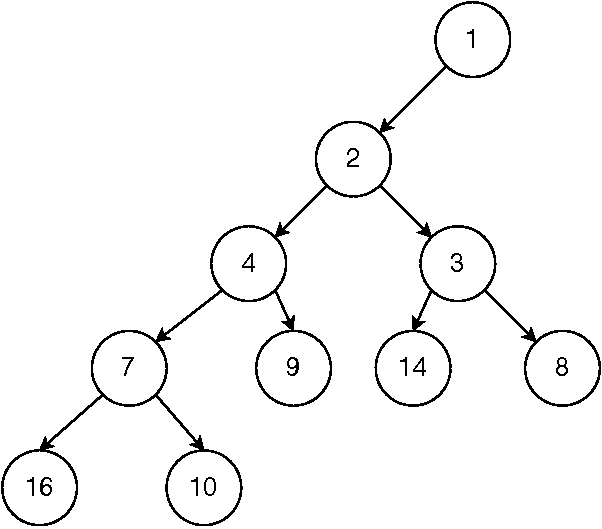
\includegraphics[scale=0.5]{img/leftist-tree.ps}
    \caption{A Leftist tree built from list $\{9, 4, 16, 7, 10, 2, 14, 3, 8, 1\}$.}
    \label{fig:leftist-tree}
   \end{center}
\end{figure}

The following example Haskell code gives reference implementation
for the Leftist tree operations.

\lstset{language=Haskell}
\begin{lstlisting}
insert h x = merge (Node 1 x E E) h

findMin (Node _ x _ _) = x

deleteMin (Node _ _ l r) = merge l r

fromList = foldl insert E
\end{lstlisting}

% ================================================================
%                 Heap sort
% ================================================================
\subsection{Heap sort by Leftist Heap}
\index{Leftist heap!heap sort}

With all the basic operations defined, it's straightforward to
implement heap sort. We can firstly turn the list into a Leftist
heap, then continuously extract the minimum
element from it.

\be
sort(L) = heapSort(build(L))
\ee

\be
heapSort(H) = \left \{
  \begin{array}
  {r@{\quad:\quad}l}
  \phi & H = \phi \\
  \{top(H)\} \cup heapSort(pop(H)) & otherwise
  \end{array}
\right.
\ee

Because pop is logarithm operation, and it is recursively called $n$ times,
this algorithm takes $O(n \lg n)$ time in total. The following Haskell
example program implements heap sort with Leftist tree.

\lstset{language=Haskell}
\begin{lstlisting}
heapSort = hsort . fromList where
    hsort E = []
    hsort h = (findMin h):(hsort $ deleteMin h)
\end{lstlisting} %$



% ================================================================
%                 Skew Heap
% ================================================================

\subsection{Skew heaps}
\label{skew-heap}
\index{Skew heap}

Leftist heap leads to quite unbalanced structure sometimes. Figure \ref{fig:unbalanced-leftist-tree}
shows one example. The Leftist tree is built by folding on
list $\{16, 14, 10, 8, 7, 9, 3, 2, 4, 1\}$.

\begin{figure}[htbp]
   \begin{center}
   	  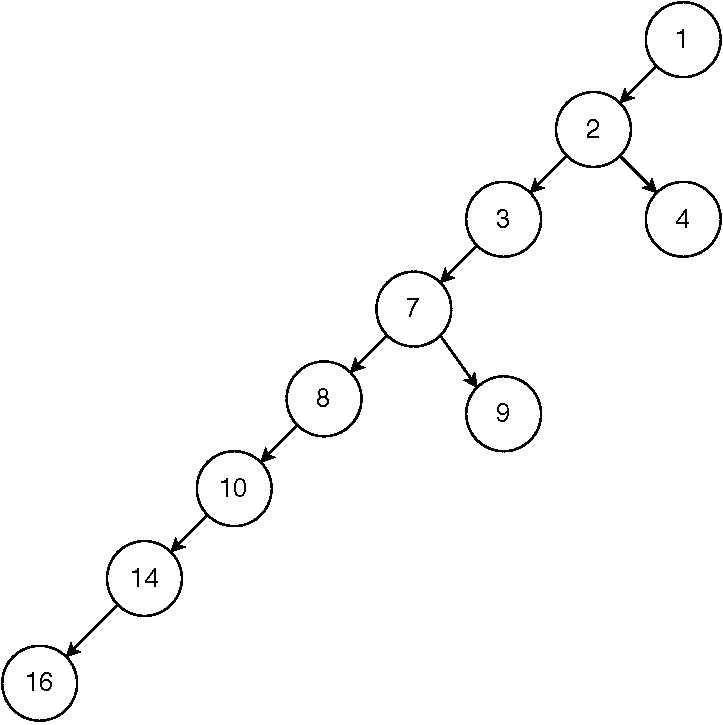
\includegraphics[scale=0.3]{img/unbalanced-leftist-tree.ps}
    \caption{A very unbalanced Leftist tree build from list $\{16, 14, 10, 8, 7, 9, 3, 2, 4, 1\}$.}
    \label{fig:unbalanced-leftist-tree}
   \end{center}
\end{figure}

Skew heap (or {\em self-adjusting heap}) simplifies Leftist heap realization
and intends to solve the balance issue\cite{wiki-skew-heap} \cite{self-adjusting-heaps}.

When construct the Leftist heap, we swap the left and right children during merge
if the rank on left side is less than the right side. This comparison-and-swap strategy
doesn't work when either sub tree has only one child. Because
in such case, the rank of the sub tree is always 1 no matter how
big it is. A `Brute-force' approach is to swap the left and right children
every time when merge. This idea leads to Skew heap.

\subsubsection{Definition of Skew heap}

Skew heap is the heap realized with Skew tree. Skew tree is a special
binary tree. The minimum element is stored in root. Every sub tree is
also a skew tree.

It needn't keep the rank (or $S$-value) field. We can reuse the
binary tree definition for Skew heap. The tree is either empty,
or in a pre-order form $(k, L, R)$. Below Haskell code defines
Skew heap like this.

\lstset{language=Haskell}
\begin{lstlisting}
data SHeap a = E -- Empty
             | Node a (SHeap a) (SHeap a) -- element, left, right
\end{lstlisting}

\subsubsection{Merge}
\index{Skew heap!merge}
\index{Skew heap!insertion}
\index{Skew heap!top}
\index{Skew heap!pop}

The merge algorithm tends to be very simple.
When merge two non-empty Skew
trees, we compare the roots, and pick the smaller
one as the new root, then the other tree contains the bigger
element is merged onto one sub tree, finally,
the tow children are swapped. Denote $H_1 = (k_1, L_1, R_1)$
and $H_2 =(k_2, L_2, R_2)$ if they are not empty.
if $k_1 < k_2$ for instance, select $k_1$ as the new root. We can
either merge $H_2$ to $L_1$, or merge $H_2$ to $R_1$.
Without loss of generality, let's merge to $R_1$.
And after swapping the two children, the final result
is $(k_1, merge(R_1, H_2), L_1)$. Take account of
edge cases, the merge algorithm is defined as the
following.

\be
merge(H_1, H_2) = \left \{
  \begin{array}
  {r@{\quad:\quad}l}
  H_1 & H_2 = \phi \\
  H_2 & H_1 = \phi \\
  (k_1, merge(R_1, H_2), L_1) & k_1 < k_2 \\
  (k_2, merge(H_1, R_2), L_2) & otherwise
  \end{array}
\right.
\ee

All the rest operations, including insert, top and pop are all
realized as same as the Leftist heap by using merge, except that
we needn't the rank any more.

Translating the above algorithm into Haskell yields the following
example program.

\lstset{language=Haskell}
\begin{lstlisting}
merge E h = h
merge h E = h
merge h1@(Node x l r) h2@(Node y l' r') =
    if x < y then Node x (merge r h2) l
    else Node y (merge h1 r') l'

insert h x = merge (Node x E E) h

findMin (Node x _ _) = x

deleteMin (Node _ l r) = merge l r
\end{lstlisting}

Different from the Leftist heap, if we feed ordered list to Skew heap, it can build a
fairly balanced binary tree as illustrated in figure \ref{fig:skew-tree}.

\begin{figure}[htbp]
   \begin{center}
   	  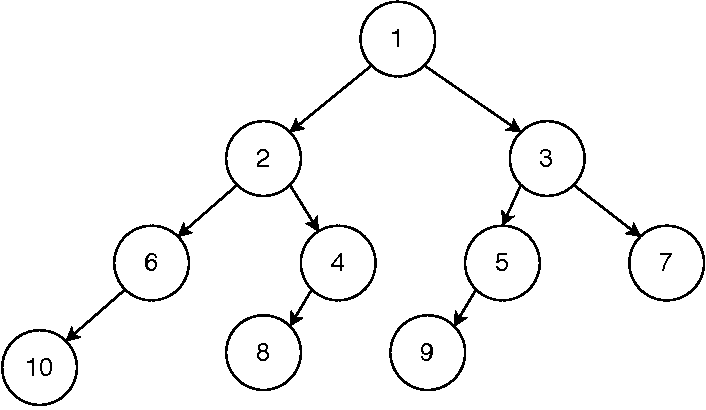
\includegraphics[scale=0.5]{img/skew-tree.ps}
    \caption{Skew tree is still balanced even the input is an ordered list $\{1, 2, ..., 10\}$.}
    \label{fig:skew-tree}
   \end{center}
\end{figure}


% ================================================================
%                 Splay Heap
% ================================================================

\section{Splay heap}
\label{splayheap}
\index{Splay heap}

The Leftist heap and Skew heap show the fact that it's quite possible to realize
heap data structure with explicit binary tree.
Skew heap gives one method to solve the tree balance problem. Splay heap
on the other hand, use another method to keep the tree balanced.

The binary trees used in Leftist heap and Skew heap
are not Binary Search tree (BST). If we turn the underground
data structure to binary search tree, the minimum(or maximum)
element is not root any more. It takes $O(\lg n)$ time
to find the minimum(or maximum) element.

Binary search tree becomes inefficient if it isn't well
balanced. Most operations degrade to $O(n)$ in the worst case.
Although red-black tree can be used to realize
binary heap, it's overkill. Splay tree provides a light weight
implementation with acceptable dynamic balancing result.


% ================================================================
%                 Definition
% ================================================================
\subsection{Definition}

Splay tree uses cache-like approach. It keeps rotating the current
access node close to the top, so that the node can be accessed fast
next time. It defines such kinds of operation as ``Splay''. For the
unbalanced binary search tree, after several splay operations, the
tree tends to be more and more balanced. Most basic operations of
Splay tree perform in amortized $O(\lg n)$ time. Splay tree was invented
by Daniel Dominic Sleator and Robert Endre Tarjan in 1985\cite{wiki-splay-tree}
\cite{self-adjusting-trees}.

\subsubsection{Splaying}
\index{Splay heap!splaying}

There are two methods to do splaying. The first one need deal
with many different cases, but can be implemented fairly easy with
pattern matching. The second one has a uniformed form, but the implementation
is complex.

Denote the node currently being accessed as $X$, the parent node as $P$,
and the grand parent node as $G$ (If there are).  There are 3 steps for
splaying. Each step contains 2 symmetric cases. For illustration
purpose, only one case is shown for each step.

\begin{itemize}
\item {\em Zig-zig step.} As shown in figure \ref{fig:zig-zig}, in this case,
$X$ and $P$ are children on the same side of $G$, either both on left or right. By
rotating 2 times, $X$ becomes the new root.

\begin{figure}[htbp]
  \centering
  \subfloat[$X$ and $P$ are both left children or both right children.]{\includegraphics[scale=0.4]{img/zig-zig-a.ps}}
  \subfloat[$X$ becomes new root after rotating 2 times.]{\includegraphics[scale=0.4]{img/zig-zig-b.ps}}
  \caption{Zig-zig case.} \label{fig:zig-zig}
\end{figure}

\item {\em Zig-zag step.} As shown in figure \ref{fig:zig-zag}, in this
case, $X$ and $P$ are children on different sides. $X$ is on the left,
$P$ is on the right. Or $X$ is on the right, $P$ is on the left.
After rotation, $X$ becomes the new root, $P$ and $G$ are siblings.

\begin{figure}[htbp]
  \centering
  \subfloat[$X$ and $P$ are children on different sides.]{\includegraphics[scale=0.4]{img/zig-zag-a.ps}}
  \subfloat[$X$ becomes new root. $P$ and $G$ are siblings.]{\includegraphics[scale=0.4]{img/zig-zag-b.ps}}
  \caption{Zig-zag case.} \label{fig:zig-zag}
\end{figure}

\item {\em Zig step.} As shown in figure \ref{fig:zig}, in this case,
$P$ is the root, we rotate the tree, so that $X$ becomes new root.
This is the last step in splay operation.

\begin{figure}[htbp]
  \centering
  \subfloat[$P$ is the root.]{\includegraphics[scale=0.4]{img/zig-a.ps}}
  \subfloat[Rotate the tree to make $X$ be new root.]{\includegraphics[scale=0.4]{img/zig-b.ps}}
  \caption{Zig case.} \label{fig:zig}
\end{figure}

\end{itemize}

Although there are 6 different cases, they can be handled in the
environments support pattern matching. Denote the non-empty binary tree
in form $T=(L, k, R)$,. when access key $Y$ in tree $T$, the splay
operation can be defined as below.

\be
splay(T, X) = \left \{
  \begin{array}
  {r@{\quad:\quad}l}
  (a, X, (b, P, (c, G, d))) & T = (((a, X, b), P, c), G, d), X = Y \\
  (((a, G, b), P, c), X, d) & T= (a, G, (b, P, (c, X, d))), X = Y \\
  ((a, P, b), X, (c, G, d)) & T = (a, P, (b, X, c), G, d), X = Y \\
  ((a, G, b), X, (c, P, d)) & T = (a, G, ((b, X, c), P, d)), X = Y \\
  (a, X, (b, P, c)) & T = ((a, X, b), P, c), X = Y \\
  ((a, P, b), X, c) & T = (a, P, (b, X, c)), X = Y \\
  T &  otherwise
  \end{array}
\right.
\ee

The first two clauses handle the 'zig-zig' cases; the next two
clauses handle the 'zig-zag' cases; the last two clauses handle
the zig cases. The tree aren't changed for all other situations.

The following Haskell program implements this splay function.

\lstset{language=Haskell}
\begin{lstlisting}
data STree a = E -- Empty
             | Node (STree a) a (STree a) -- left, key, right

-- zig-zig
splay t@(Node (Node (Node a x b) p c) g d) y =
    if x == y then Node a x (Node b p (Node c g d)) else t
splay t@(Node a g (Node b p (Node c x d))) y =
    if x == y then Node (Node (Node a g b) p c) x d else t
-- zig-zag
splay t@(Node (Node a p (Node b x c)) g d) y =
    if x == y then Node (Node a p b) x (Node c g d) else t
splay t@(Node a g (Node (Node b x c) p d)) y =
    if x == y then Node (Node a g b) x (Node c p d) else t
-- zig
splay t@(Node (Node a x b) p c) y = if x == y then Node a x (Node b p c) else t
splay t@(Node a p (Node b x c)) y = if x == y then Node (Node a p b) x c else t
-- otherwise
splay t _ = t
\end{lstlisting}

With splay operation defined, every time when insert a new key,
we call the splay function to adjust the tree.
If the tree is empty, the result is a leaf; otherwise we compare this key
with the root, if it is less than the root, we recursively insert it into
the left child, and perform splaying after that; else the key is inserted
into the right child.

\be
insert(T, x) = \left \{
  \begin{array}
  {r@{\quad:\quad}l}
  (\phi, x, \phi) & T = \phi \\
  splay((insert(L, x), k, R), x) & T = (L, k, R), x < k \\
  splay(L, k, insert(R, x)) & otherwise
  \end{array}
  \right.
\ee

The following Haskell program implements this insertion algorithm.

\lstset{language=Haskell}
\begin{lstlisting}
insert E y = Node E y E
insert (Node l x r) y
    | x > y     = splay (Node (insert l y) x r) y
    | otherwise = splay (Node l x (insert r y)) y
\end{lstlisting}

Figure \ref{fig:splay-result} shows the result of using this function.
It inserts the ordered elements $\{1, 2, ..., 10\}$
one by one to the empty tree. This would build a very poor result
which downgrade to linked-list with normal binary search tree.
The splay method creates more balanced result.

\begin{figure}[htbp]
  \centering
  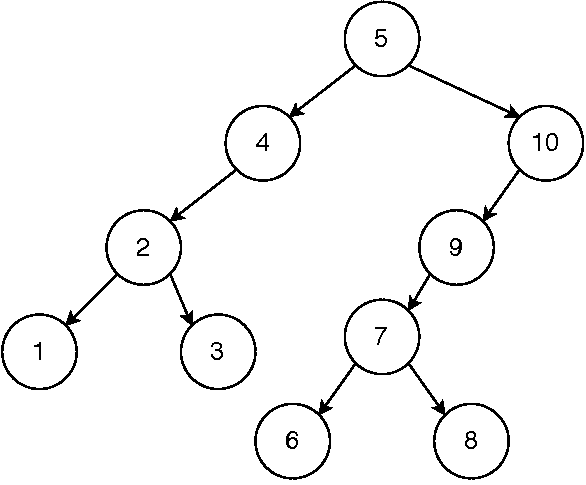
\includegraphics[scale=0.5]{img/splay-tree.ps}
  \caption{Splaying helps improving the balance.}
  \label{fig:splay-result}
\end{figure}

Okasaki found a simple rule for Splaying \cite{okasaki-book}.
Whenever we follow
two left branches, or two right branches continuously, we rotate
the two nodes.

Based on this rule, splaying can be realized in such a way.
When we access node for a key $x$ (can be during the process of
inserting a node, or looking up a node, or deleting a node), if
we traverse two left branches or two right branches, we
partition the tree in two parts $L$ and $R$, where $L$ contains all
nodes smaller than $x$, and $R$ contains all the rest.
We can then create a new tree (for instance in insertion),
with $x$ as the root, $L$ as the left child, and $R$ being the right child.
The partition process is recursive, because it will splay
its children as well.

\be
partition(T, p) = \left \{
  \begin{array}
  {r@{\quad:\quad}l}
  (\phi, \phi) & T = \phi \\
  (T, \phi) & T = (L, k, R) \land R = \phi \\
  ((L, k, L'), k', A, B) & \begin{array}{l} \\
                             T = (L, k, (L', k', R')) \\
                             k < p, k' < p \\
                             (A, B) = partition(R', p)
                           \end{array} \\
  ((L, k, A), (B, k', R')) & \begin{array}{l} \\
                               T = (L, K, (L', k', R')) \\
                               k < p \leq k' \\
                               (A, B) = partition(L', p) \\ \\
                             \end{array} \\
  (\phi, T) & T = (L, k, R) \land L = \phi \\
  (A, (L', k', (R', k, R)) & \begin{array}{l} \\
                               T = ((L', k', R'), k, R) \\
                               p \leq k, p \leq k' \\
                               (A, B) = partition(L', p)
                             \end{array} \\
  ((L', k', A), (B, k, R)) & \begin{array}{l} \\
                               T = ((L', k', R'), k, R) \\
                               k' \leq p \leq k \\
                               (A, B) = partition(R', p)
                             \end{array}
  \end{array}
  \right.
\ee

Function $partition(T, p)$ takes a tree $T$, and a pivot $p$ as arguments.
The first clause is edge case. The partition result for empty is
a pair of empty left and right trees. Otherwise, denote the tree
as $(L, k, R)$. we need compare the pivot $p$ and the root $k$.
If $k < p$, there are two sub-cases. one is trivial case that
$R$ is empty. According to the property of binary search tree,
All elements are less than $p$, so the result pair is $(T, \phi)$;
For the other case, $R = (L', k', R')$, we need further compare
$k'$ with the pivot $p$. If $k' < p$ is also true, we recursively
partition $R'$ with the pivot, all the elements less than $p$ in
$R'$ is held in tree $A$, and the rest is in tree $B$. The
result pair can be composed with two trees, one is $((L, k, L'), k', A)$;
the other is $B$. If the key of the right sub tree is not less than
the pivot, we recursively partition $L'$ with the pivot to give
the intermediate pair $(A, B)$, the final pair trees can be
composed with $(L, k, A)$ and $(B, k', R')$. There are symmetric
cases for $p \leq k$. They are handled in the last three clauses.

Translating the above algorithm into Haskell yields the following partition
program.

\begin{lstlisting}
partition E _ = (E, E)
partition t@(Node l x r) y
    | x < y =
        case r of
          E -> (t, E)
          Node l' x' r' ->
              if x' < y then
                  let (small, big) = partition r' y in
                  (Node (Node l x l') x' small, big)
              else
                  let (small, big) = partition l' y in
                  (Node l x small, Node big x' r')
    | otherwise =
        case l of
          E -> (E, t)
          Node l' x' r' ->
              if y < x' then
                  let (small, big) = partition l' y in
                  (small, Node l' x' (Node r' x r))
              else
                  let (small, big) = partition r' y in
                  (Node l' x' small, Node big x r)
\end{lstlisting}

% ================================================================
%                 Basic heap operations
% ================================================================
\index{Splay heap!insertion}
Alternatively, insertion can be realized with $partition$ algorithm.
When insert a new element $k$ into
the splay heap $T$, we can first partition the heap into two trees, $L$ and $R$. Where
$L$ contains all nodes smaller than $k$, and $R$ contains the rest.
We then construct a new node, with $k$ as the root and $L$, $R$ as the children.

\be
insert(T, k) = (L, k, R), (L, R) = partition(T, k)
\ee

The corresponding Haskell example program is as the following.

\lstset{language=Haskell}
\begin{lstlisting}
insert t x = Node small x big where (small, big) = partition t x
\end{lstlisting}

\subsubsection{Top and pop}
\index{Splay heap!top}
\index{Splay heap!pop}
Since splay tree is just a special binary search tree, the minimum
element is stored in the left most node. We need keep traversing
the left child to realize the top operation. Denote the none empty
tree $T=(L, k, R)$, the $top(T)$ function can be defined as below.

\be
top(T) = \left \{
  \begin{array}
  {r@{\quad:\quad}l}
  k & L = \phi \\
  top(L) & otherwise
  \end{array}
  \right.
\ee

This is exactly the $min(T)$ algorithm for binary search tree.

For pop operation, the algorithm need remove the minimum element from the
tree. Whenever there
are two left nodes traversed, the splaying operation should be performed.

\be
pop(T) = \left \{
  \begin{array}
  {r@{\quad:\quad}l}
  R & T = (\phi, k, R) \\
  (R', k, R) & T = ((\phi, k', R'), k, R) \\
  (pop(L'), k', (R', k, R)) & T = ((L', k', R'), k, R)
  \end{array}
  \right.
\ee

Note that the third clause performs splaying without explicitly call
the $partition$ function. It utilizes the property of binary
search tree directly.

Both the top and pop algorithms are bound to $O(\lg n)$ time because
the splay tree is balanced.

The following Haskell example programs implement the top and pop
operations.

\lstset{language=Haskell}
\begin{lstlisting}
findMin (Node E x _) = x
findMin (Node l x _) = findMin l

deleteMin (Node E x r) = r
deleteMin (Node (Node E x' r') x r) = Node r' x r
deleteMin (Node (Node l' x' r') x r) = Node (deleteMin l') x' (Node r' x r)
\end{lstlisting}

\subsubsection{Merge}
\index{Splay heap!merge}
Merge is another basic operation for heaps as it is widely used in Graph algorithms. By using the $partition$ algorithm, merge can be realized in $O(\lg n)$ time.

When merging two splay trees, for non-trivial case, we can take the root of the first tree as the new root, then partition the second tree with this new root as the pivot. After that we recursively merge
the children of the first tree to the partition result. This algorithm is defined as the following.

\be
merge(T_1, T_2) = \left \{
  \begin{array}
  {r@{\quad:\quad}l}
  T_2 & T_1 = \phi \\
  (merge(L, A), k, merge(R, B)) & T_1 = (L, k, R), (A, B) = partition(T_2, k)
  \end{array}
  \right.
\ee

If the first heap is empty, the result is definitely the second heap. Otherwise,
denote the first splay heap as $(L, k, R)$, we partition $T_2$ with $k$ as the
pivot to yield $(A, B)$, where $A$ contains all the elements in $T_2$ which are
less than $k$, and $B$ holds the rest. We next recursively merge $A$ with $L$;
and merge $B$ with $R$ as the new children for $T_1$.

Translating the definition to Haskell gives the following example program.

\lstset{language=Haskell}
\begin{lstlisting}
merge E t = t
merge (Node l x r) t = Node (merge l l') x (merge r r')
    where (l', r') = partition t x
\end{lstlisting}

% ================================================================
%                 Heap sort
% ================================================================
\subsection{Heap sort}

Since the internal implementation of the Splay heap is completely
transparent to the heap interface, the heap sort algorithm can
be reused. It means that the heap sort algorithm is generic no
matter what the underground data structure is.

% ================================================================
%                 Short summary
% ================================================================
\section{Notes and short summary}

In this chapter, we define binary heap more general
so that as long as the heap property is maintained, all binary
representation of data structures can be used to implement binary heap.

This definition doesn't limit to the popular array based binary
heap, but also extends to the explicit binary heaps including Leftist
heap, Skew heap and Splay heap. The array based binary heap
is particularly convenient for the imperative implementation
because it intensely uses random index access which can be mapped to
a completely binary tree. It's hard to find directly functional
counterpart in this way.

However, by using explicit binary tree, functional implementation
can be achieved, most of them have $O(\lg n)$ worst case
performance, and some of them even reach $O(1)$ amortize time.
Okasaki in \cite{okasaki-book} shows detailed analysis of these data
structures.

In this chapter, only purely functional realization for Leftist heap,
Skew heap, and Splay heap are explained, they can all be realized
in imperative approaches.

It's very natural to extend the concept from binary tree to
$k$-ary ($k$-way) tree, which leads to other useful heaps such as
Binomial heap, Fibonacci heap and pairing heap. They are introduced
in the following chapters.

% ================================================================
%                 Exercise
% ================================================================
\begin{Exercise}
\begin{itemize}
\item Realize the imperative Leftist heap, Skew heap, and Splay heap.
\end{itemize}
\end{Exercise}


\begin{thebibliography}{99}

\bibitem{CLRS}
Thomas H. Cormen, Charles E. Leiserson, Ronald L. Rivest and Clifford Stein. ``Introduction to Algorithms, Second Edition''. The MIT Press, 2001. ISBN: 0262032937.

\bibitem{wiki-heap}
Heap (data structure), Wikipedia. http://en.wikipedia.org/wiki/Heap\_(data\_structure)

\bibitem{wiki-heapsort}
Heapsort, Wikipedia. http://en.wikipedia.org/wiki/Heapsort

\bibitem{okasaki-book}
Chris Okasaki. ``Purely Functional Data Structures''. Cambridge university press, (July 1, 1999), ISBN-13: 978-0521663502

\bibitem{rosetta-heapsort}
Sorting algorithms/Heapsort. Rosetta Code. http://rosettacode.org/wiki/Sorting\_algorithms/Heapsort

\bibitem{wiki-leftist-tree}
Leftist Tree, Wikipedia. http://en.wikipedia.org/wiki/Leftist\_tree

\bibitem{brono-book}
Bruno R. Preiss. Data Structures and Algorithms with Object-Oriented Design Patterns in Java. http://www.brpreiss.com/books/opus5/index.html

\bibitem{TAOCP}
Donald E. Knuth. ``The Art of Computer Programming. Volume 3: Sorting and Searching.''. Addison-Wesley Professional;
2nd Edition (October 15, 1998). ISBN-13: 978-0201485417. Section 5.2.3 and 6.2.3

\bibitem{wiki-skew-heap}
Skew heap, Wikipedia. http://en.wikipedia.org/wiki/Skew\_heap

\bibitem{self-adjusting-heaps}
Sleator, Daniel Dominic; Jarjan, Robert Endre. ``Self-adjusting heaps'' SIAM Journal on Computing 15(1):52-69. doi:10.1137/0215004 ISSN 00975397 (1986)

\bibitem{wiki-splay-tree}
Splay tree, Wikipedia. http://en.wikipedia.org/wiki/Splay\_tree

\bibitem{self-adjusting-trees}
Sleator, Daniel D.; Tarjan, Robert E. (1985), ``Self-Adjusting Binary Search Trees'', Journal of the ACM 32(3):652 - 686, doi: 10.1145/3828.3835

\bibitem{NIST}
NIST, ``binary heap''. http://xw2k.nist.gov/dads//HTML/binaryheap.html

\end{thebibliography}

\ifx\wholebook\relax \else
\end{document}
\fi
